\chapter{Тестирање брзине извршавања У/И операција}

Како би се увидела предност \textit{Lustre} фајл система у односу на NFS фајл систем, вршено је мерење брзине извршавања У/И операција на \textit{Мedflow} кластеру високих перформанси који користи оба наведена фајл система. Тестирање је вршено помоћу три различите апликације:


\begin{itemize}
\item \textit{Iozone} - апликација намењена тестирању перформанси улазно-излазних операција,
\item \texttt{dd} - једноставан UNIX системски алат за конверзију и копирање фајлова,
\item \textit{Game of Life} - "реална" апликација која поред У/И операција поседује и делове у којима се интензивно рачуна.
\end{itemize}

\section{Хардверска конфигурација кластера}

Medflow кластер је састављен од HP Proliant SL230s Gen8 и HP Proliant SL250s Gen8 радних чворова, заснованих на Intel® Xeon® E5-2600 (Sandy Bridge) процесорима. Кластер се састоји од следећих компоненти:

\begin{itemize}

\item 18 радних чворова HP Proliant SL230s Gen8 са 2 Intel® Xeon® E5-2660 процесора (2.2GHz – 8 cores - 20MB L3 cache - 95W) и  64GB RAM меморије.
\item 4 радна чвора P Proliant SL250s са 2 Intel® Xeon® E5-2670 (2.6GHz – 8 cores - 20MB L3 cache - 115W) процесора и  64GB RAM меморије. Сваки од ових чворова садржи и 1 GPU NVIDIA Tesla
M2090 6G графичку картицу.
\item Једног \textit{Mellanox Infiniband} QDR свич преко кога су повезани чворови.  
\item Једног управљачког сервера DL380pGen8 који омогућава пријаву на систем.
\item Једног управљачког сервера DL380pGen8 који омогућава функционисање паралелног фајл система.
\item Система за складиштење података који садржи 1 \textit{HP P2000 G3 Modular Smart Array System} повезан на управљачки сервер, што даје укупно 12TB простора (6 HDD дискова по 2TB). Низ је конфигурисан као RAID ниво 6. Сви чворови могу приступити овим дисковима помоћу \textit{Lustre} протокола.
\end{itemize}
 
 \begin{figure}[h!]
   \centering
       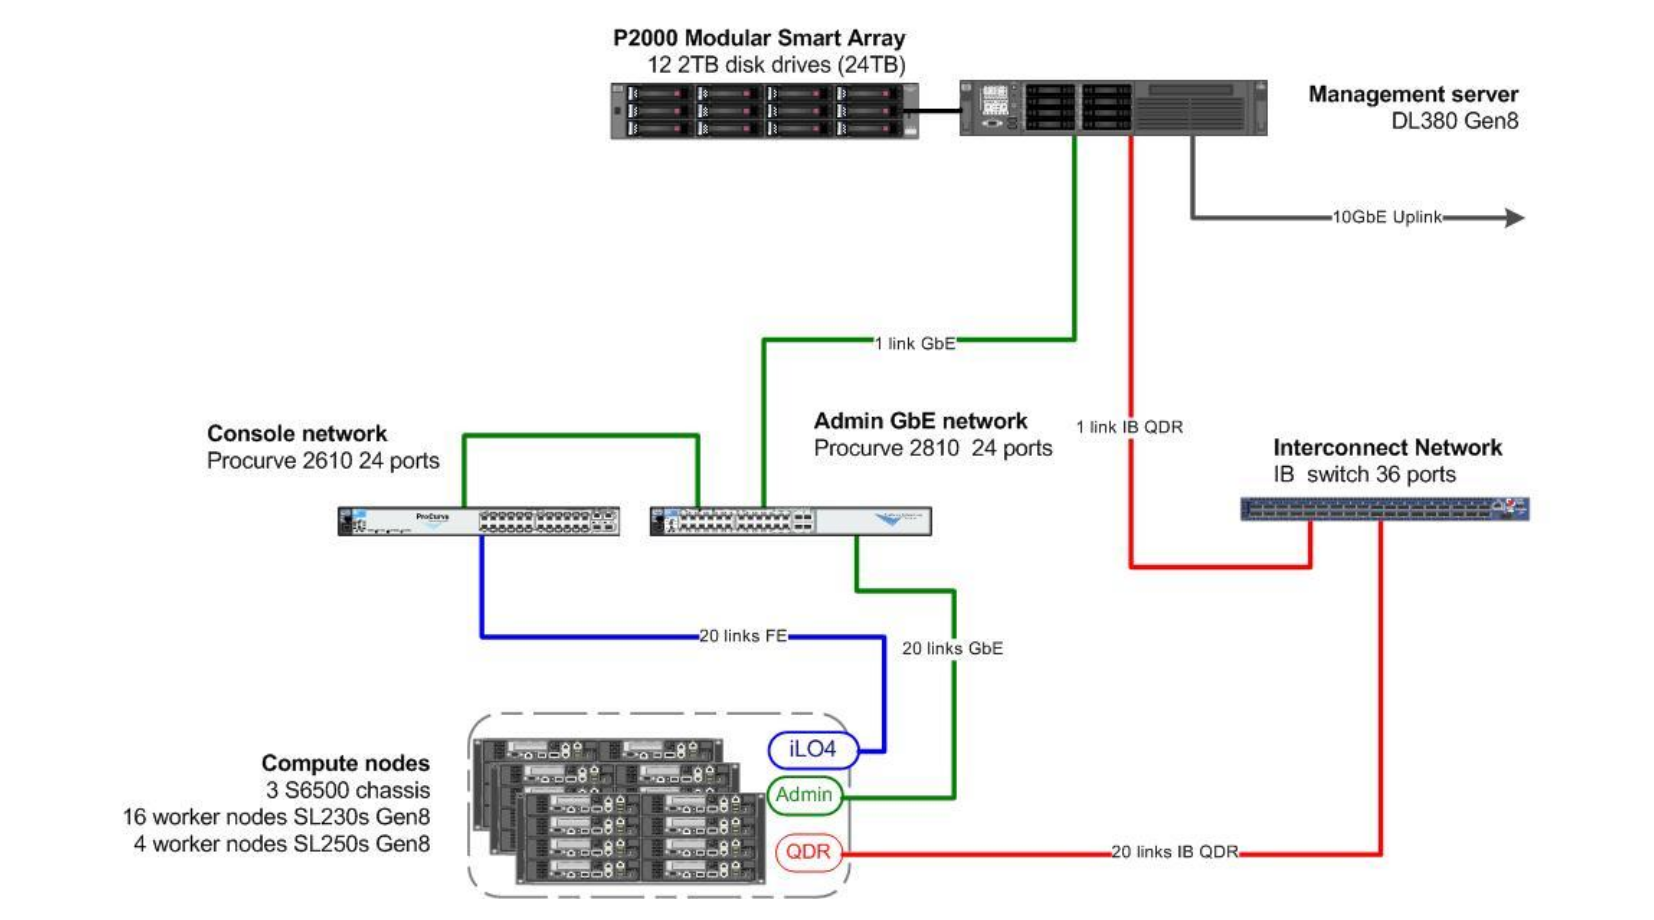
\includegraphics[width=1\textwidth]{slike/medflow.png}\\[1cm]
   \caption{Компоненте кластера}
 \end{figure}
 
Кластер је конфигурисан са Linux Kernel 2.6 на свим чворовима. Scientific Linux 6.6 64-bit је инсталиран како на управљачком чвору, тако и на радним чворовима. Ресурсима кластера се управља помоћу \textit{TORQUE} и \textit{Maui} сервиса. Први је намењен контроли и управљању кластер пословима, док је други распоређивач. 
 
Програмско окружење је засновано на OpenMPI библиотекама за Linux оперативни систем. На кластеру је инсталирана OpenMPI верзија 1.6.5. Треба нагласити и да је \gls{NFS} фајл систем инсталиран постављен само на једном диску, док Lustre користи цео RAID6 низ. 

\section{Iozone тестирање}
\textit{Iozone} је алат за мерење брзине У/И операција фајл система. Он генерише и мери трајање великог броја операција са фајловима. \textit{Iozone} може бити  инсталиран на великом броју архитектура и такође може радити у оквиру многих оперативних система. Тестирање се врши кроз следеће операције:

\begin{itemize}
\item \textit{Write} - мери брзину уписа података у нови фајл.
\item \textit{Re-write} - мери брзину уписа у фајл који већ постоји
\item \textit{Read} - мери брзину читања из фајла
\item \textit{Re-read} - мери брзину читања из фајла који је претходно прочитан
\item \textit{Random read} - мери брзину читања из фајла са насумичним приступом локацијама унутар фајла
\item \textit{Random write} - мери брзину писања у фајл са насумичним приступом локацијама унутар фајла
\item \textit{Random mix} - мери брзину писања и читања из фајла са насумичним приступом локацијама унутар фајла
\item \textit{Backwards read} - мери брзину читања из фајла уназад
\item \textit{Record rewrite} - мери брзину писања података у одређени део фајла
\item \textit{Strided read} - мери брзину читања из фајла са тачно одређеним параметрима
\item \textit{Fwrite} - мери брзину писања у фајл помоћу функције \texttt{fwrite()}
\item \textit{Fread} - мери брзину читања из фајла помоћу функције \texttt{fread()}
\item \textit{Freread} - мери поновно читања из фајла  помоћу функције \texttt{fwrite()}
\end{itemize}


\subsection{Инсталација и покретање програма}

\textit{Iozone} програм се инсталира помоћу следећих команди:
\begin{lstlisting}[style=nonumbers,frame=single,language=C, caption= Инсталација Iozone]
wget http://www.iozone.org/src/current/iozone3_394.tar

tar xvf iozone3_394.tar 

cd iozone3_394/src/current

make

make linux

\end{lstlisting}

Овај програм је могуће покренути и помоћу великог број параметара. Конкретни параметри који су коришћени за тестирање на кластеру имају следеће значење:

\begin{itemize}
\item \texttt{-b назив фајла} - генерисање Excel излазног фајла
\item \texttt{-c} - мери и време које је потребно за функцију \textit{ close()}
\item \texttt{-I} - користи \textit{DIRECT I/O} заставицу за све фајл операције
\item \texttt{-о} - уписује синхроно на диск. \textit{Iozone} отвара фајл са \textit{O\_SYNC} заставицом
\item \texttt{-r} - oдређује величину записа у килобајтима
\item \texttt{-s} - oдређује величину фајла који се користи за тестирање 
\end{itemize}
Програм се покреће помоћу команде:
\begin{verbatim}
./iozone -s 25000000 -r 1024 -I -c -o -b output.xls
\end{verbatim}

Резултати програма се могу видети у фајлу \textit{output.xls}.

  \begin{figure}[h!]
    \centering
        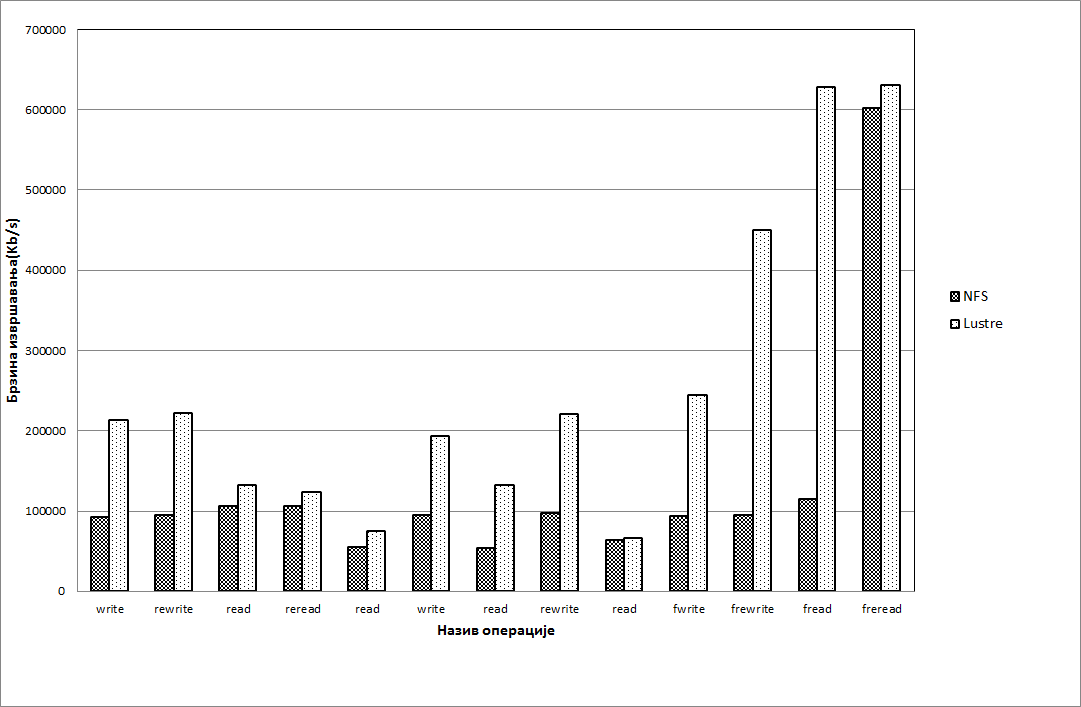
\includegraphics[width=0.85\textwidth]{slike/results/iozone.png}\\[1cm]
    \caption{\textit{Iozone} резултати}
  \end{figure}
  
Посматрајући резултате представљене на Слици 4.2, закључујемо да је брзина извршавања улазно/излазних операција \textit{Lustre} фајл система значајно већа у односу на брзину NFS система без обзира на врсту операције која се извршава. Највећа разлика у брзини се уочава код теста који користи \texttt{fread()} команду, док је најмања разлика у брзини при извршавању операције обичног читања.
  
\section{Тестирање помоћу \texttt{dd} програма }

\texttt{dd} је једноставан алат који служи за писање и читање блокова података диска. Он такође мери и брзину којом је операција извршена.

Параметри командне линије су:

\begin{itemize}
\item \texttt{if} - улазни фајл
\item \texttt{of} - излазни фајл
\item \texttt{bs} - величина блока
\item \texttt{count} - број блокова
\end{itemize}
Програм за упис у фајл  се покреће командом:
\begin{verbatim}
dd if=/dev/zero bs=1M count=16384 of=file_16GB
\end{verbatim}
а за читање из фајла:
\begin{verbatim}
dd if=file_16GB bs=1M of=/dev/null
\end{verbatim}
Добијени су следећи резултати:
\begin{figure}[H]
   \centering
       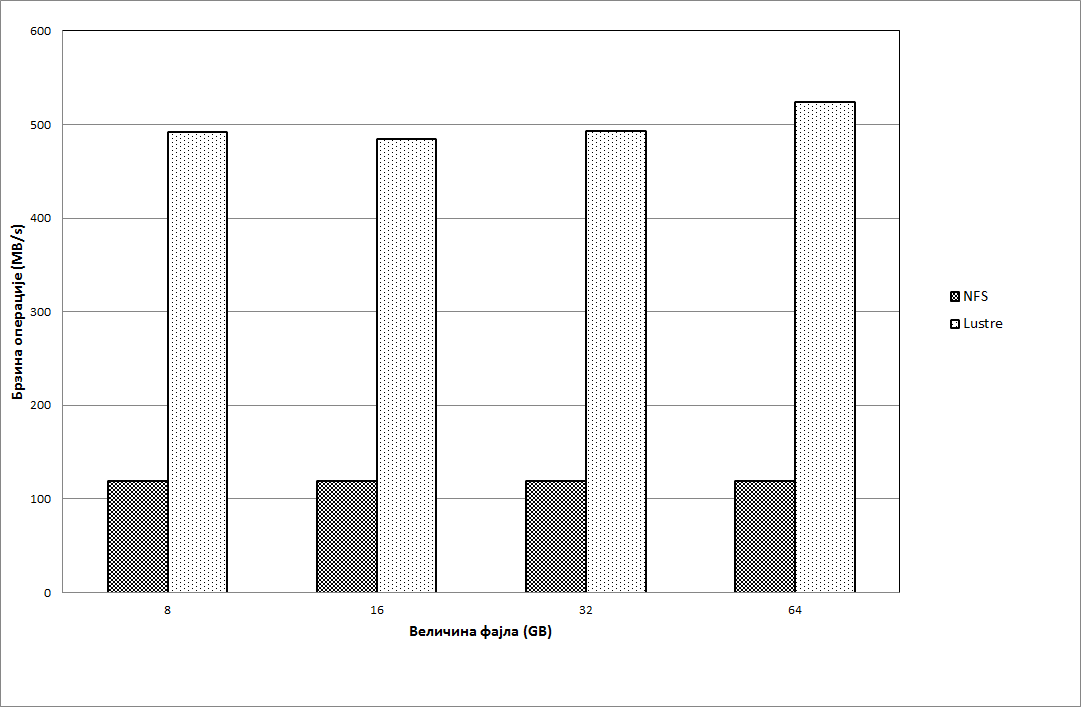
\includegraphics[width=0.85\textwidth]{slike/results/dd_read_speed.png}\\[1cm]
   \caption{Резултати брзине читања}
\end{figure} 
\begin{figure}[H]
    \centering
        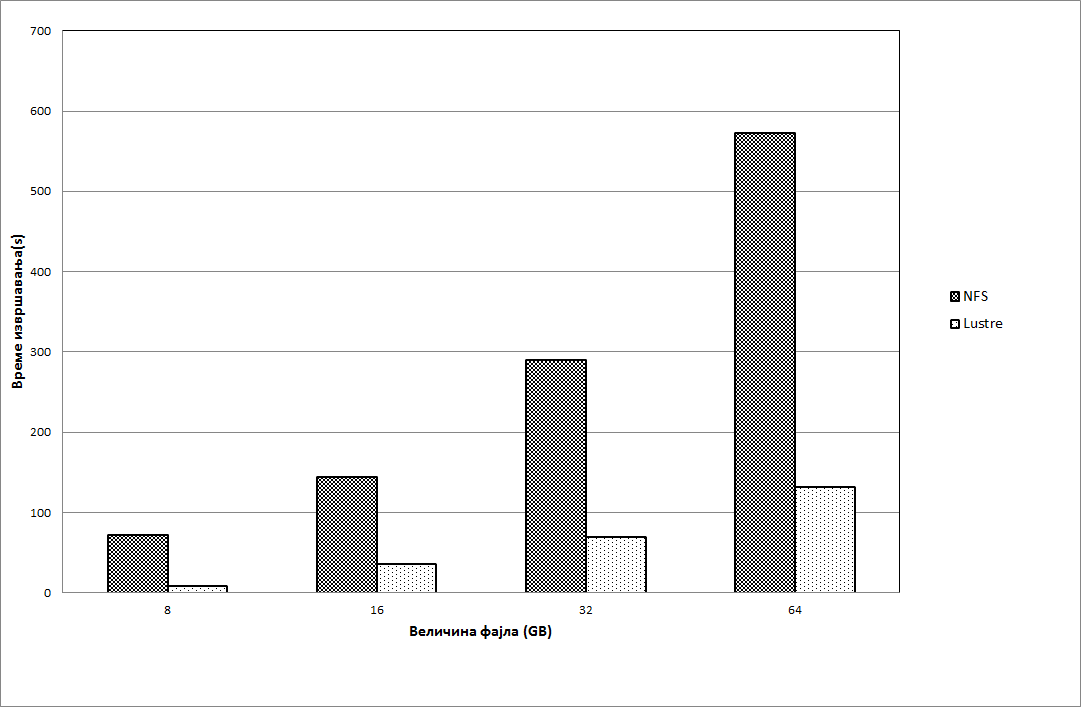
\includegraphics[width=0.85\textwidth]{slike/results/dd_read_time.png}\\[1cm]
    \caption{Резултати времена извршавања програма читања}
\end{figure}  
\begin{figure}[H]
     \centering
         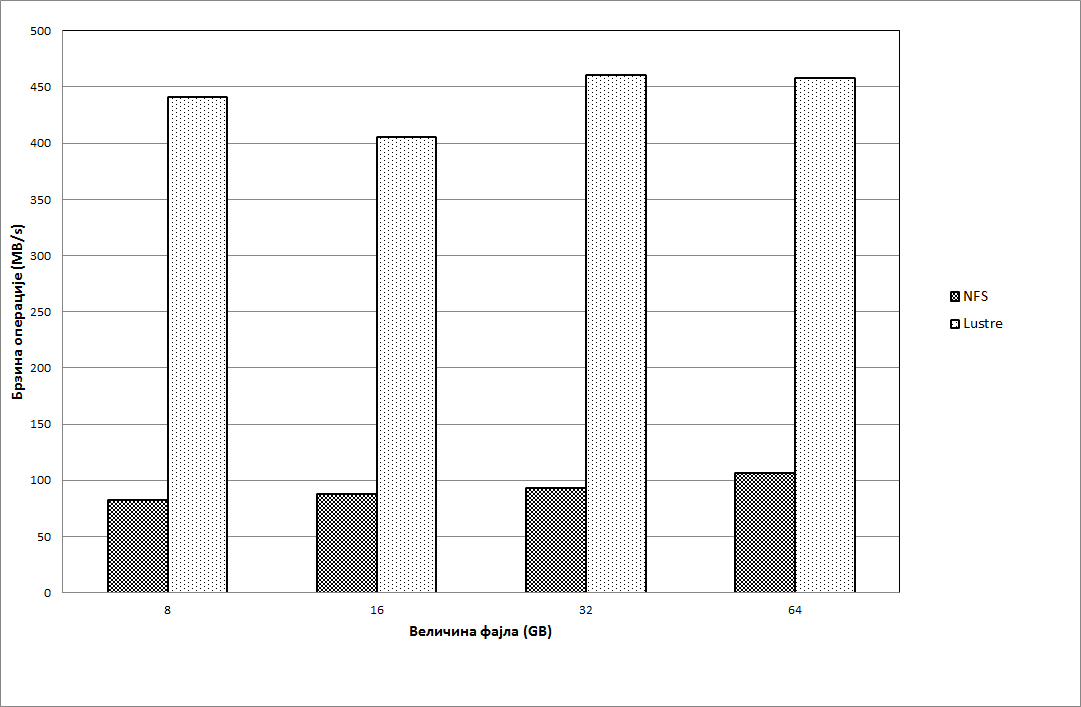
\includegraphics[width=0.85\textwidth]{slike/results/dd_write_speed.png}\\[1cm]
     \caption{Резултати брзине писања}
\end{figure}   
\begin{figure}[H]
      \centering
          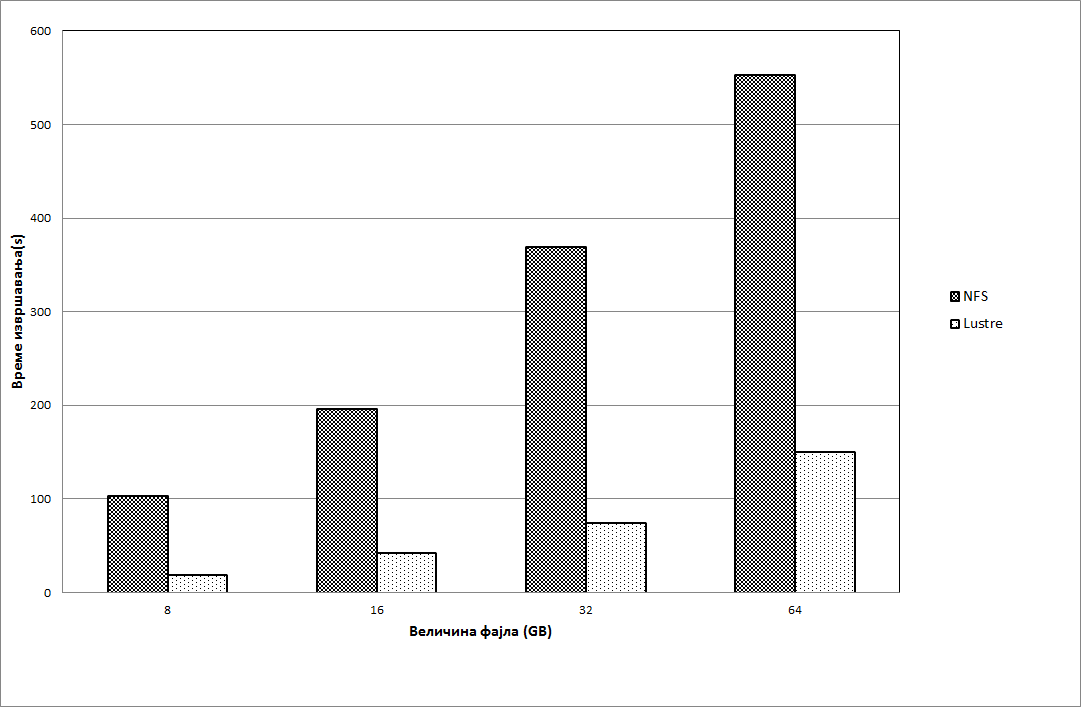
\includegraphics[width=0.85\textwidth]{slike/results/dd_write_time.png}\\[1cm]
      \caption{Резултати времена извршавања програма писања}
\end{figure}   
 
Анализирајући слике 2.3 и 2.5 на којима је приказана брзина читања односно писања закључује се да је \textit{Lustre} фајл систем вишеструко бржи независно од величине фајла који се чита, односно који се уписује.
На сликама 2.4 и 2.6, које приказују време извршавања програма читања, односно писања, уочава се да је разлика у овим фајл системима већа уколико је величина фајла већа. Што је фајл већи, \textit{Lustre} показује већу супериорност у односу на NFS.

\section{Game of Life}
\textit{Game of Life} је најпознатији пример ћелијског аутомата који је осмислио британски математичар Џон Конвеј 1970 године. Ова игра је игра без играча, што значи да је њена еволуција одређена првобитним стањем. 
За тестирање је коришћен \textit{Game of life} MPI-2 програм, коме су дадате функције читања и уписа стања ћелија, које се позивају након сваког корака симулације. Програм је покретан на \textit{Lustre} фајл систему, а затим са истим улазним параметрима на NFS фајл систему. \textit{Game of Life} је погодан јер не захтева додатне корисничке уносе након покретања програма. Матрицa помоћу којe сe прате стања ћелија могуће је декомпоновати независно од броја процеса. Подешавајући улазне параметре, мења се и величина података коју је потребно уписати у фајл.

\subsection{Правила}
\textit{Game of Life} је представљена бесконачном дводимензионалном мрежом квадратних ћелија од којих је свака у једном од два могућа стања: активном или пасивном. Свака ћелија је у односу са осам суседних ћелија, које су са њом повезане хоризонтално, вертикално или дијагонално. Са сваким кораком у времену јављају се следеће транзиције:

\begin{itemize}
\item Било која активна ћелија која има мање од две активне ћелије које су јој суседне постаје пасивна.
\item Било која жива ћелија са више од три активне ћелије које су јој суседне постаје пасивна да не би дошло до пренатрпаности.
\item Било која ћелија са две или три активне суседне ћелије живи, не мења се и преноси на следећу генерацију.
\item Било која пасивна ћелија која има три активне суседне ћелије постаће и сама активна.
\end{itemize}

Почетни модел представља почетну популацију система. Свака популација је чиста функција претходне. Правило се наставља примењивати узастопно ради креирања наредних генерација.

\subsection{Порекло}
Конвеј је био заинтересован за проблем представљен четрдесетих година двадесетог века од стране реномираног математичара Џон ван Нојмана који је покушавао да пронађе машину која би могла да изради копије себе и успео је када је пронашао математички модел за такву машину са веома компликованим правилима на правоугаоној мрежи. Игра је доживела своје прво јавно појављивање у октобру 1970-е у колумни „Математичке игре“ под називом фантастичне комбинације Џона Конвеја. Са теоретске тачке гледишта је занимљиво, јер има моћ универзалне Тјурингове машине. Све што се може алгоритамски обрачунавати може се израчунати и са Конвејевом \textit{Game of Life}.

Још од њеног објављивања, \textit{Game of Life} је привукла велико интересовање због изненађујућих начина на који се обрасци могу развијати. Занимљиво је за физичаре, биологе, економисте, математичаре, филозофе, научнике и остале да посматрају начин на који се сложени обрасци могу појавити из примене веома једноставних правила. На пример, филозоф и научник Даниел Ц. Денет је користио Конвејеве \textit{Game of Life}  интензивно да илуструје могућу еволуцију сложених филозофских конструкција, као што су свест и слободна воља, од релативно једноставног скупа детерминистичких физичких закона који регулишу наш сопствени универзум.
Популарност Конвејеве игре је потпомогнута њеном појавом баш у време појаве нове генерације јефтиних мини рачунара који су пуштени у промет. Игра може да се активира ноћу, током сати када су машине иначе неискоришћене. За многе, \textit{Game of Life} је једноставно програмирање, изазов, забаван начин да губимо циклусе процесора. За неке, међутим, \textit{Game of Life} је више филозофске конотације.

\section{Опис програма}
Програм је написан у C програмском језику користећи MPI функције. На почетку програма се учитавају параметри програма. 

Улазни параметри програма су:
\begin{itemize}
\item начин генерисања почетне популације 
\item број процеса
\item величина квадратне матрице
\item број итерација
\item начин уписа - уколико је 0 онда се матрица уписује у 1 фајл. Уколико је 1 онда сваки процес свој део матрице уписује у свој фајл.
\end{itemize}
Свака ћелија је представљена као поље у матрици. На основу унетих параметара, креира се и генерише почетна популација. У свакој итерацији се на основу објашњених правила рачуна вредност поља у матрици, а затим се на основу начина уписа резултат уписује у фајл или фајлове. Као резултат програма, добија се време које је потребно да се програм изврши.

На кластеру програм се покреће помоћу следеће скрипте:

\begin{lstlisting}[style=nonumbers,frame=single,language=C, caption=Скрипта за покретање програма на кластеру]
#!/bin/sh
#PBS -N lustre_mpi
#PBS -q batch
#PBS -l nodes=8:ppn=8

module load openmpi-pmf-x86_64
chmod 755 mpi_lustre
mpirun ./mpi_lustre random 128 128 1 
\end{lstlisting}

пис и читање из фајла се врши у свакој итерацији. У зависности од начина уписа, потребно је отворити фајл или фајлове за читање и писање. Уколико је \texttt{write\_type} једнак нули онда сви процеси вршe операције са једном фајлом, у супротном сваки процес има посебан фајл из ког чита и у који уписује.

\begin{lstlisting}[style=nonumbers,frame=single,language=C, caption=Део кода за отварање фајлова за читање и писање]

	MPI_File thefile;
	int nnp, *myold;
	MPI_Status status;	

    if (write_type == 0) 
    {
        MPI_File_open(MPI_COMM_WORLD, filename,
                      MPI_MODE_CREATE | MPI_MODE_RDWR,
                      MPI_INFO_NULL, &thefile);

        MPI_File_set_view(thefile, nnp * id * sizeof(int),
                          MPI_INT, MPI_INT, "native", MPI_INFO_NULL);
    }
    else 
    {
        MPI_File_open(MPI_COMM_SELF, filename,
                      MPI_MODE_RDWR | MPI_MODE_CREATE, MPI_INFO_NULL, &thefile);
    } 
\end{lstlisting}

\begin{lstlisting}[style=nonumbers,frame=single,language=C, caption=Функције за читање и писање у фајл]
	MPI_File_read(thefile, myold, nnp, MPI_INT, &status);
	
	MPI_File_write(thefile, myold, nnp, MPI_INT, MPI_STATUS_IGNORE);
\end{lstlisting}
где се садржај низа \texttt{myold} чита или уписује у фајл \texttt{thefile}.

\newpage
\section{Резултати тестирања}

На графиконима је приказано време извршавања у зависности од улазих параметара. 
 
 \begin{figure}[H]
   \centering
       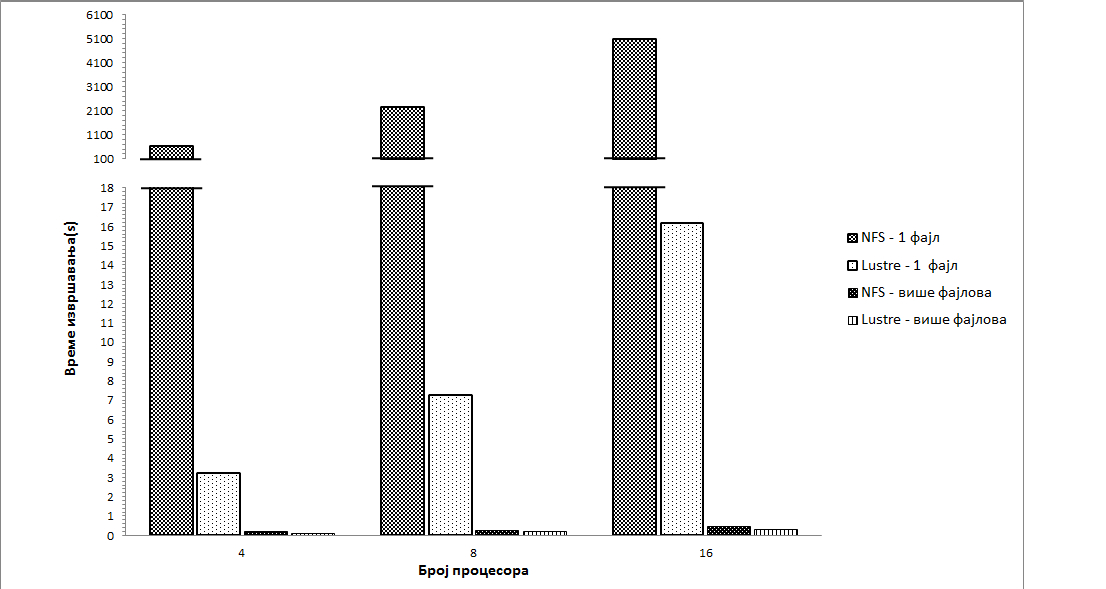
\includegraphics[width=1\textwidth]{slike/results/32_32.png}\\[1cm]
   \caption{Матрица 32x32, 32 итерација}
 \end{figure}
 
  \begin{figure}[H]
    \centering
        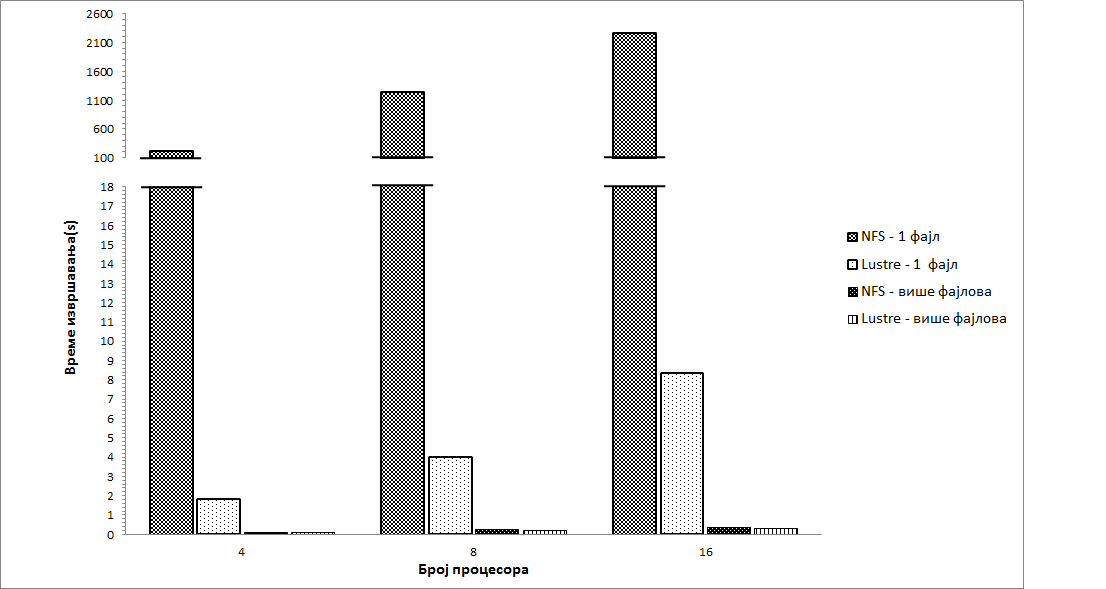
\includegraphics[width=1\textwidth]{slike/results/32_64.png}\\[1cm]
    \caption{Матрица 32x32, 64 итерација}
  \end{figure}
 
    \begin{figure}[H]
      \centering
          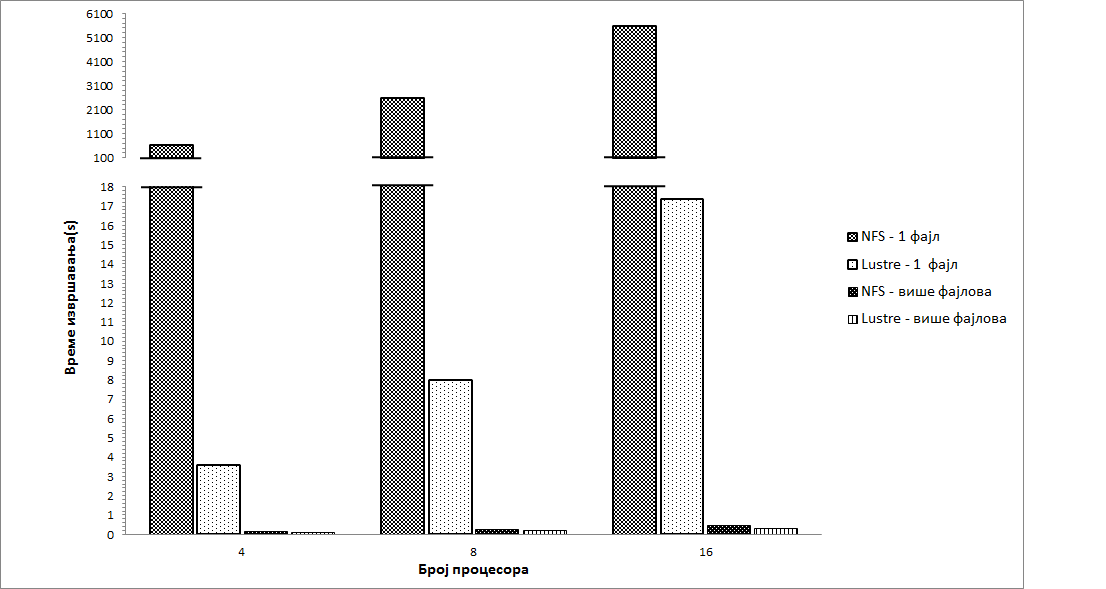
\includegraphics[width=1\textwidth]{slike/results/32_128.png}\\[1cm]
      \caption{Матрица 32x32, 128 итерација}
    \end{figure}
   
    \begin{figure}[H]
      \centering
          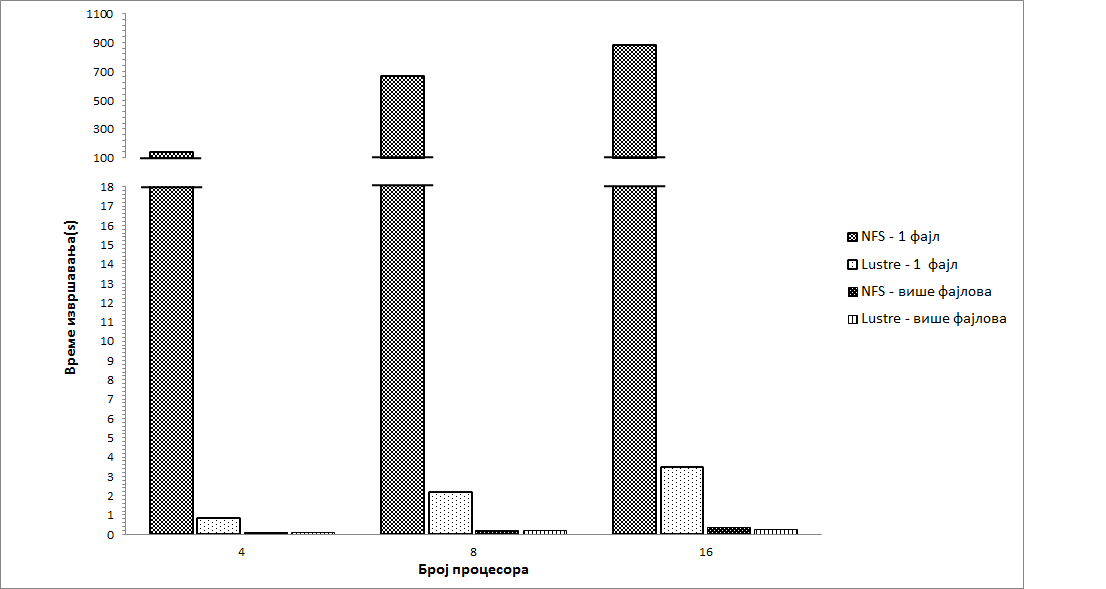
\includegraphics[width=1\textwidth]{slike/results/64_32.png}\\[1cm]
      \caption{Матрица 64x64, 32 итерација}
    \end{figure}
    
     \begin{figure}[H]
       \centering
           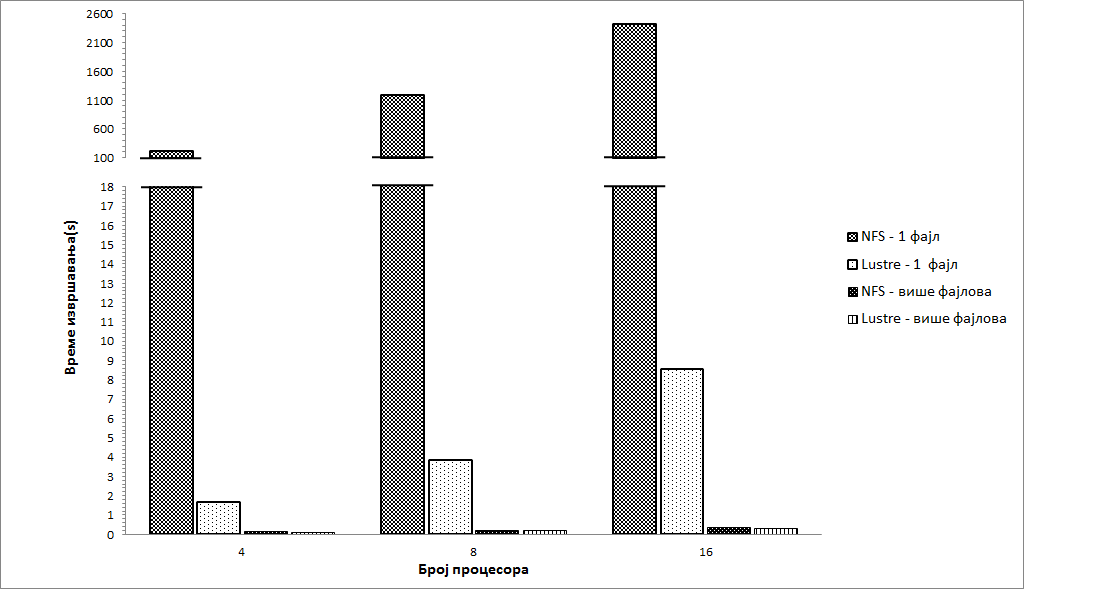
\includegraphics[width=1\textwidth]{slike/results/64_64.png}\\[1cm]
        \caption{Матрица 64x64, 64 итерација}
     \end{figure}
     
      \begin{figure}[H]
        \centering
            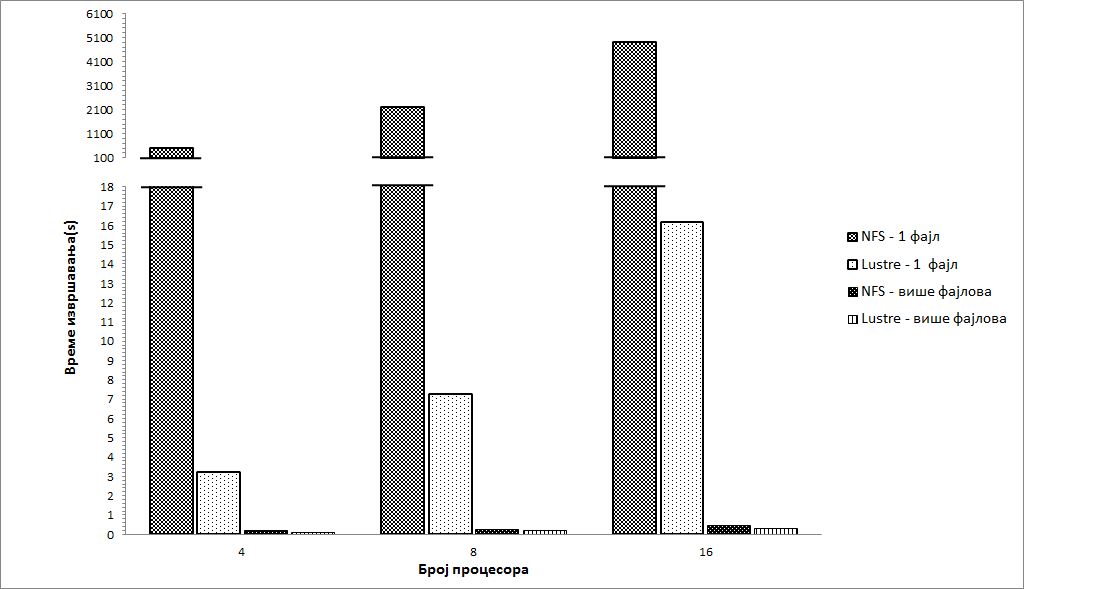
\includegraphics[width=1\textwidth]{slike/results/64_128.png}\\[1cm]
         \caption{Матрица 64x64, 128 итерација}
      \end{figure}
      
      \begin{figure}[H]
        \centering
            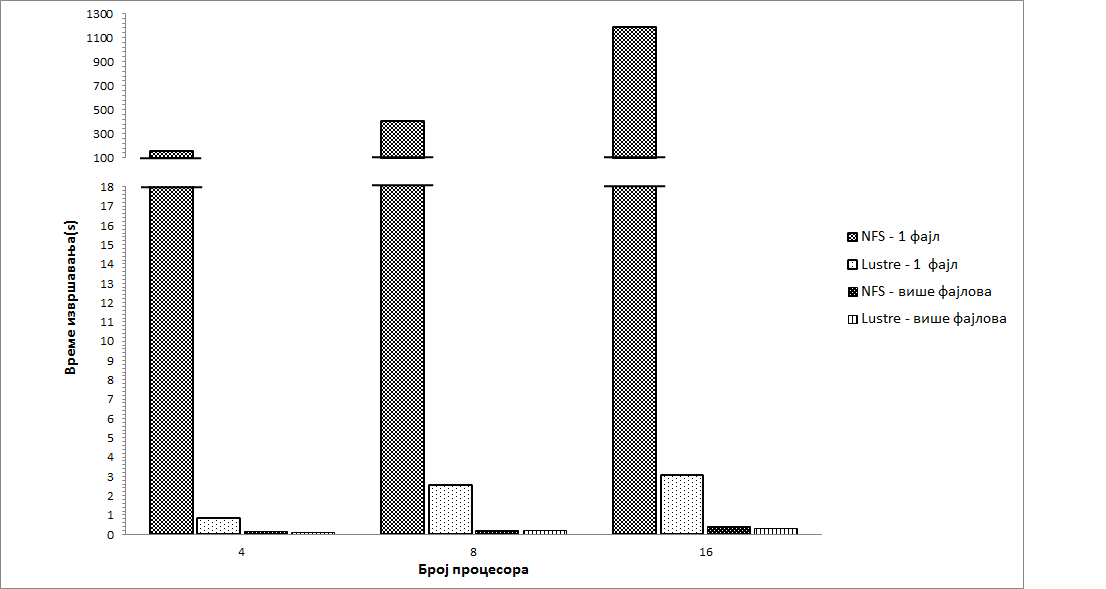
\includegraphics[width=1\textwidth]{slike/results/128_32.png}\\[1cm]
        \caption{Матрица 128x128, 32 итерација}
      \end{figure}
      
      \begin{figure}[H]
        \centering
            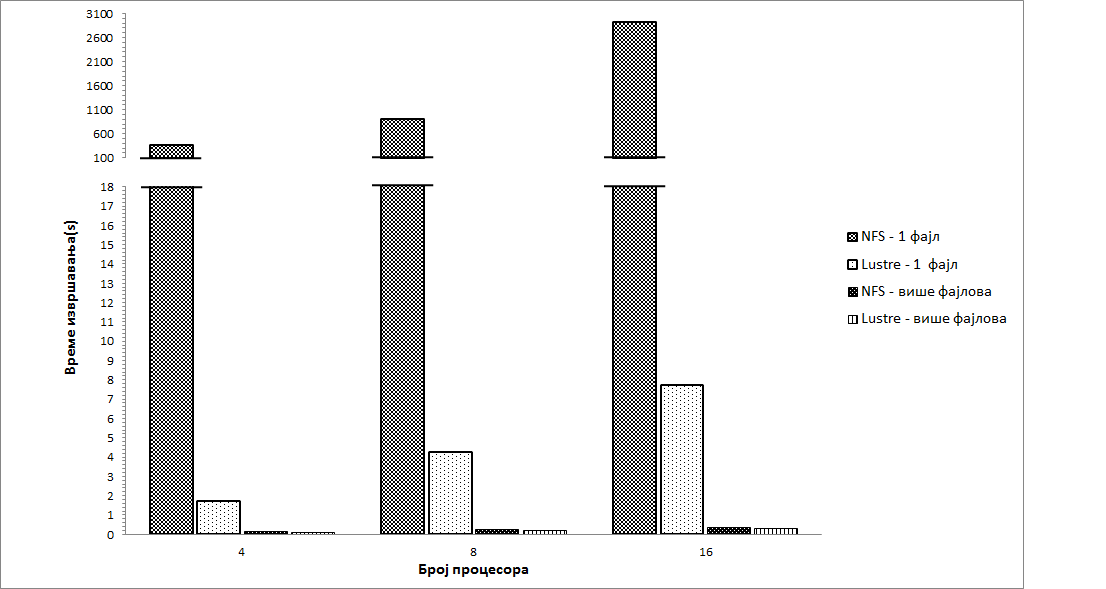
\includegraphics[width=1\textwidth]{slike/results/128_64.png}\\[1cm]
        \caption{Матрица 128x128, 64 итерација}
      \end{figure}
      
      \begin{figure}[H]
        \centering
            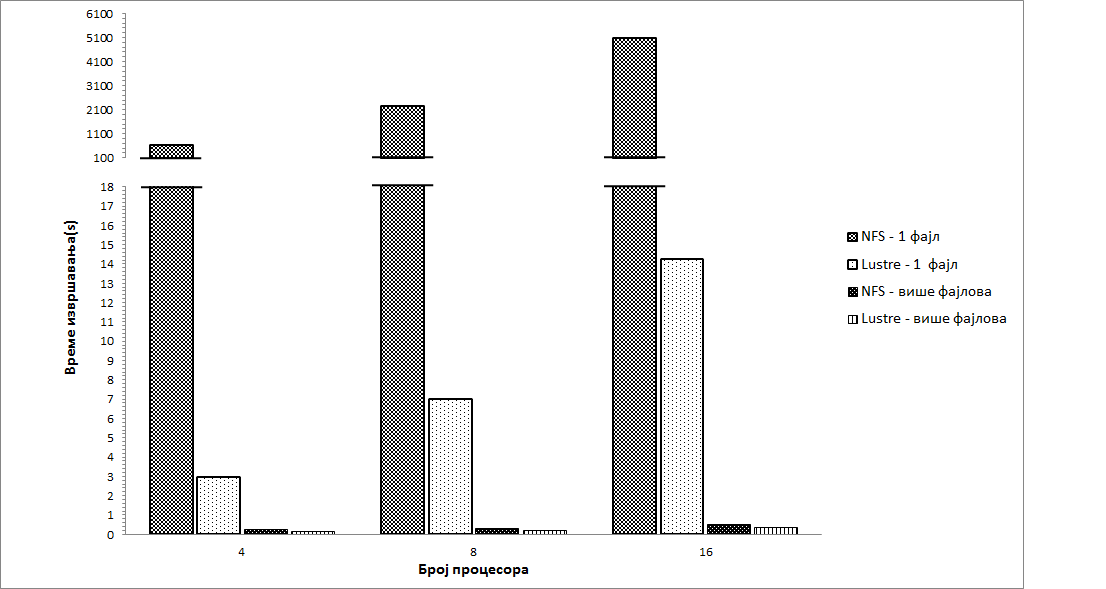
\includegraphics[width=1\textwidth]{slike/results/128_128.png}\\[1cm]
       \caption{Матрица 128x128, 128 итерација}
      \end{figure}
  
Од слике 4.7 до 4.15 приказано је време извршавања програма \textit{Game of Life} у зависности од комбинације параметара као што су: број процеса, величине матрице, број итерација и начин коришћења улазно/излазних операција. Уочава се да је време извршавања значајно мање код \textit{Lustre} фајл система, посебно када сваки процес има засебан фајл. Када сви процеси користе један фајл, \textit{Lustre} фајл систему је опет потребно мање времена него NFS фајл систему. Повећањем броја процеса ова разлика постаје уочљивија. 
Што је већа матрица и већи број итерација, то је количина података већа. Читањем и писањем већег броја података, \textit{Lustre} показује већу ефикасност. 
  
    
\chapter{Закључак}     


 Тестирањем брзина улазно/излазних операција код \textit{Lustre} фајл система и NFS добијени су резултати који показују да је  \textit{Lustre} фајл систем далеко бржи у свим типовима операција. Главни недостатак \textit{Lustre} фајл система је компликована инсталација у односу на његову алтернативу NFS. Међутим, уштеда времена у току вршења тестирања је огромна што се никако не сме занемарити. Та предност је нарочито значајна при извршавању обимних математичких операција које захтевају рад са фајловима. MPI-2 стандард са новим функцијама које омогућавају паралелне улазно/излазне операције заједно са \textit{Lustre} фајл системом чине најбољу комбинацију за паралелне програме. Обзиром да је \textit{Lustre} фајл систем доступан бесплатно, да је његов опоравак лакши у случају отказивања чврстог диска и да подржава паралелне операције са фајловима, треба му се дати апсолутна предност у односу на NFS. Једина алтернатива коју \textit{Lustre} тренутно има на тржишту је \textit{PanFS} компаније \textit{Panasas}, који се нешто лакше конфигурише и администрира, али по цену затворености кода и више цене. 
 
 
 